\documentclass[12pt,a4paper,utf8]{article}

\usepackage{xeCJK}
\usepackage{amsmath,amsthm,amssymb}
\usepackage{algorithm,algorithmic}
%\usepackage[boxed]{algorithm2e}
%\usepackage[noend]{algpseudocode}
\usepackage{hyperref}
\usepackage{graphicx}
\usepackage{xcolor}
\usepackage{float}
\usepackage{makeidx}
\usepackage{listings} 
\usepackage[numbers,sort&compress]{natbib}
\usepackage[level]{datetime}
\usepackage{indentfirst}
\usepackage{enumitem}
\usepackage{lscape}
\usepackage{pdflscape}
\usepackage{lipsum}
\usepackage{multicol}
\usepackage[top=1.5cm, bottom=2cm, outer=1.5cm, inner=1.5cm, heightrounded, marginparwidth=0cm, marginparsep=0cm]{geometry}
%\usepackage{showframe}

\renewcommand{\today}{\number\year 年 \number\month 月 \number\day 日}
\renewcommand{\refname}{参考文献}
\renewcommand{\tablename}{表}
\renewcommand{\contentsname}{目录}

\newcommand{\upcite}[1]{\textsuperscript{\textsuperscript{\cite{#1}}}}
\newcommand{\tabincell}[2]{\begin{tabular}{@{}#1@{}}#2\end{tabular}}

\definecolor{dkgreen}{rgb}{0,0.6,0}
\definecolor{gray}{rgb}{0.5,0.5,0.5}
\definecolor{mauve}{rgb}{0.58,0,0.82}
\lstset{
  language=c++,                   % the language of the code 
  basicstyle=\footnotesize,       % the size of the fonts that are used for the code
  % numbers=left,                   % where to put the line-numbers
  numberstyle=\tiny\color{gray},  % the style that is used for the line-numbers
  stepnumber=2,                   % the step between two line-numbers. If it's 1, each line 
                                  % will be numbered
  numbersep=5pt,                  % how far the line-numbers are from the code
  backgroundcolor=\color{white},  % choose the background color
  showspaces=false,               % show spaces adding particular underscores
  showstringspaces=false,         % underline spaces within strings
  showtabs=false,                 % show tabs within strings adding particular underscores
  frame=single,                   % adds a frame around the code
  rulecolor=\color{black},        % if not set, the frame-color may be changed on line-breaks within not-black text (e.g. commens (green here))
  tabsize=2,                      % sets default tabsize to 2 spaces
  captionpos=b,                   % sets the caption-position to bottom
  breaklines=true,                % sets automatic line breaking
  breakatwhitespace=false,        % sets if automatic breaks should only happen at whitespace
  % title=\lstname,                 % show the filename of files included with \lstinputlisting;
                                  % also try caption instead of title
  keywordstyle=\color{blue},      % keyword style
  commentstyle=\color{dkgreen},   % comment style
  stringstyle=\color{mauve},      % string literal style
  escapeinside={\%*}{*)},         % if you want to add LaTeX within your code
  morekeywords={*,...}            % if you want to add more keywords to the set
}

\title{第三节课习题}
\author{高洪臣}
\date{2019年6月30日}

\begin{document}

\maketitle

\noindent
\setlength{\parindent}{2em}
\setlength{\parskip}{0.3em}
\linespread{1}

\section*{第一题}

样例代码给出了使用 LM 算法来估计曲线 $y = \exp(a x^2 + bx + c)$ 参数 $a, b, c$ 的完整过程。

\begin{enumerate}

\item 请绘制样例代码中 LM 阻尼因子 $\mu$ 随着迭代变化的曲线图({\color{red}{二次修改}})

\begin{figure}[htbp] 
	\centering
	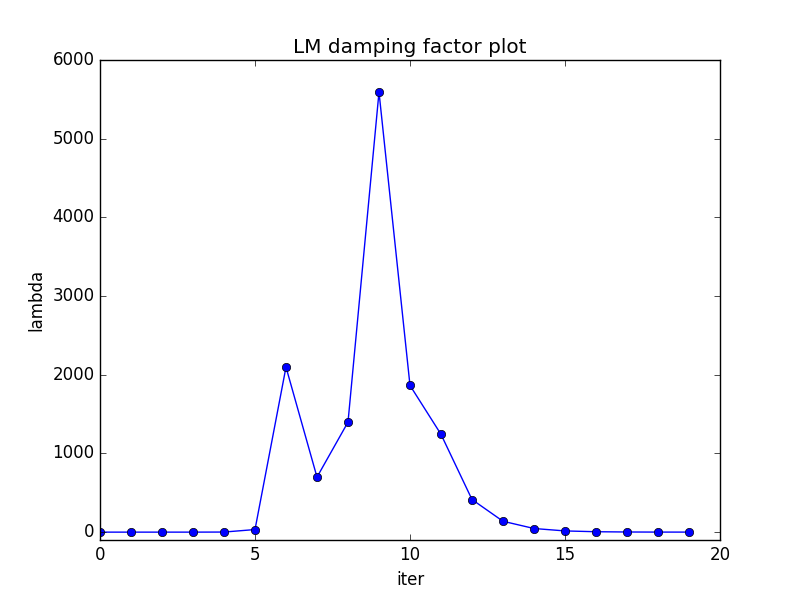
\includegraphics[width=12cm]{lm_damping_factor_new.png}
\end{figure} 

\item 将曲线函数改成 $y = a x^2 + bx + c$,请修改样例代码中残差计算,雅克比计算等函数,完成曲线参数估计

\begin{enumerate}
	\item \verb|main| 函数中修改for循环中的观测方程
	
	\begin{lstlisting}[frame=shadowbox]
	double y = a*x*x + b*x + c + n;
	\end{lstlisting}
	
	\item 修改残差计算函数为
	\begin{lstlisting}[frame=shadowbox]
	virtual void ComputeResidual() override
	{
		// 估计的参数
		Vec3 abc = verticies_[0]->Parameters();  
		// 构建残差
		residual_(0) = (abc(0)*x_*x_ + abc(1)*x_ + abc(2)) - y_;  
	}
	\end{lstlisting}
	
	\item 修改雅克比计算函数为
	\begin{lstlisting}[frame=shadowbox]
	virtual void ComputeJacobians() override
	{
		// 误差为1维,状态量 3 个,所以是 1x3 的雅克比矩阵
		Eigen::Matrix<double, 1, 3> jaco_abc;  
		jaco_abc << x_*x_, x_ , 1;
		jacobians_[0] = jaco_abc;
	}
	\end{lstlisting}
	
	\item 曲线参数估计结果
	参数真实值为 $a=1.0, b=2.0, c=1.0$,将代码中 \verb|N| 改为1000,得到参数估计值 $a=0.999588, b=2.0063, c=0.968786$
	
\end{enumerate}

\item 实现其他阻尼因子更新策略

原始程序代码实现的是\textbf{Nielsen策略},现在实现\textbf{Marquardt策略}\cite{madsen1999methods},其算法如下:

\begin{algorithm}[H]
	\label{alg:damp_marquardt}
	\caption{damping strategy by Marquardt}
	\begin{algorithmic}[1]
		\IF {$\varrho < 0.25$} 
		\STATE $\mu := \mu * 2$
		\ELSIF {$\varrho > 0.75$}
		\STATE $\mu := \mu / 3$
		\ENDIF 
	\end{algorithmic}
\end{algorithm}

根据算法~\ref{alg:damp_marquardt} 修改\verb|Problem::IsGoodStepInLM|中相关代码如下

\begin{lstlisting}[frame=shadowbox]
if(rho < 0.25) {
  currentLambda_ *= 2;
} else if (rho > 0.75) {
  currentLambda_ *= 0.3;
}

if(rho > 0) // step acceptable
  return true;
else
  return false;
\end{lstlisting}

\end{enumerate}


\section*{第二题}

公式推导,根据课程知识,完成 F, G 中如下两项的推导过程:

$$
\begin{aligned} 
\mathbf{f}_{15} &=
\frac{\partial \boldsymbol{\alpha}_{b_{i} b_{k+1}}}{\partial \delta \mathbf{b}_{k}^{g}} =
-\frac{1}{4}\left(\mathbf{R}_{b_{i} b_{k+1}}\left[\left(\mathbf{a}^{b_{k+1}}-\mathbf{b}_{k}^{a}\right)\right]_{ \times} \delta t^{2}\right)(-\delta t) \\ 
\mathbf{g}_{12} &=
\frac{\partial \boldsymbol{\alpha}_{b_{i} b_{k+1}}}{\partial \mathbf{n}_{k}^{g}} =
-\frac{1}{4}\left(\mathbf{R}_{b_{i} b_{k+1}}\left[\left(\mathbf{a}^{b_{k+1}}-\mathbf{b}_{k}^{a}\right)\right] \times \delta t^{2}\right)\left(\frac{1}{2} \delta t\right) 
\end{aligned}
$$

答:\newline

\newpage
\begin{landscape}
\thispagestyle{empty}
\setlength{\columnsep}{1cm}
\setlength{\columnseprule}{1pt} 
\def\columnseprulecolor{\color{black}}
\begin{multicols}{2}
$$
\begin{aligned}
\mathbf{f}_{15} 
&=
\frac{\partial \boldsymbol{\alpha}_{b_{i} b_{k+1}}}{\partial \delta \mathbf{b}_{k}^{g}} \\
&=
\frac{\partial (\boldsymbol{\alpha}_{b_{i} b_{k}}+\boldsymbol{\beta}_{b_{i} b_{k}} \delta t+\frac{1}{2} \mathbf{a} \delta t^{2})}{\partial \delta \mathbf{b}_{k}^{g}} \\ 
&=
\frac{1}{2} \frac{\partial \mathbf{a} \delta t^{2}}{\partial \delta \mathbf{b}_{k}^{g}} \\
&=
\frac{1}{4} \frac{\partial 
\left(\mathbf{q}_{b_{i} b_{k}}\left(\mathbf{a}^{b_{k}}-\mathbf{b}_{k}^{a}\right)+\mathbf{q}_{b_{i} b_{k+1}}\left(\mathbf{a}^{b_{k+1}}-\mathbf{b}_{k}^{a}\right)\right)\delta t^{2}}
{\partial \delta \mathbf{b}_{k}^{g}} \\
&=
\frac{1}{4} \frac{\partial 
\mathbf{q}_{b_{i} b_{k}} \otimes\left[\begin{array}{c}{1} \\ {\frac{1}{2} \omega \delta t}\end{array}\right] \left(\mathbf{a}^{b_{k+1}}-\mathbf{b}_{k}^{a}\right)\delta t^{2}}
{\partial \delta \mathbf{b}_{k}^{g}} \\
&=
\frac{1}{4} \frac{\partial 
\mathbf{q}_{b_{i} b_{k}} \otimes\left[\begin{array}{c}{1} \\ {\frac{1}{2} \omega \delta t}\end{array}\right] \otimes\left[\begin{array}{c}{1} \\ {-\frac{1}{2} \delta \mathbf{b}_{k}^{g} \delta t}\end{array}\right] \left(\mathbf{a}^{b_{k+1}}-\mathbf{b}_{k}^{a}\right) \delta t^{2}}
{\partial \delta \mathbf{b}_{k}^{g}} \\
&=
\frac{1}{4} \frac{\partial 
\mathbf{R}_{b_{i} b_{k+1}} \exp \left(\left[-\delta \mathbf{b}_{k}^{g} \delta t\right]_{ \times}\right)\left(\mathbf{a}^{b_{k+1}}-\mathbf{b}_{k}^{a}\right) \delta t^{2}}
{\partial \delta \mathbf{b}_{k}^{g}} \\
&=
\frac{1}{4} \frac{\partial 
\mathbf{R}_{b_{i} b_{k+1}}\left(\mathbf{I}+\left[-\delta \mathbf{b}_{k}^{g} \delta t\right]_{ \times}\right)\left(\mathbf{a}^{b_{k+1}}-\mathbf{b}_{k}^{a}\right) \delta t^{2}}
{\partial \delta \mathbf{b}_{k}^{g}} \\
&=
\frac{1}{4} \frac{\partial 
\mathbf{R}_{b_{i} b_{k+1}}\left[-\delta \mathbf{b}_{k}^{g} \delta t\right]_{ \times}\left(\mathbf{a}^{b_{k+1}}-\mathbf{b}_{k}^{a}\right) \delta t^{2}}
{\partial \delta \mathbf{b}_{k}^{g}} \\
&=
-\frac{1}{4} \frac{\partial 
\mathbf{R}_{b_{i} b_{k+1}}\left(\left[\left(\mathbf{a}^{b_{k+1}}-\mathbf{b}_{k}^{a}\right) \delta t^{2}\right]_{ \times}\right)\left(-\delta \mathbf{b}_{k}^{g} \delta t\right)}
{\partial \delta \mathbf{b}_{k}^{g}} \\
&=
-\frac{1}{4} 
\mathbf{R}_{b_{i} b_{k+1}}\left(\left[\left(\mathbf{a}^{b_{k+1}}-\mathbf{b}_{k}^{a}\right) \right]_{\times}\delta t^{2}\right)\left(-\delta t\right)
\end{aligned}
$$

$$
\begin{aligned} 
\mathbf{g}_{12} 
&=
\frac{\partial \boldsymbol{\alpha}_{b_{i} b_{k+1}}}{\partial \mathbf{n}_{k}^{g}} \\
&=
\frac{\partial (\boldsymbol{\alpha}_{b_{i} b_{k}}+\boldsymbol{\beta}_{b_{i} b_{k}} \delta t+\frac{1}{2} \mathbf{a} \delta t^{2})}{\partial \mathbf{n}_{k}^{g}} \\ 
&=
\frac{1}{2} \frac{\partial \mathbf{a} \delta t^{2}}{\partial \mathbf{n}_{k}^{g}} \\
&=
\frac{1}{4} \frac{\partial 
	\left(\mathbf{q}_{b_{i} b_{k}}\left(\mathbf{a}^{b_{k}}-\mathbf{b}_{k}^{a}\right)+\mathbf{q}_{b_{i} b_{k+1}}\left(\mathbf{a}^{b_{k+1}}-\mathbf{b}_{k}^{a}\right)\right)\delta t^{2}}
{\partial \mathbf{n}_{k}^{g}} \\
&=
\frac{1}{4} \frac{\partial 
	\mathbf{q}_{b_{i} b_{k}} \otimes\left[\begin{array}{c}{1} \\ {\frac{1}{2} \omega \delta t}\end{array}\right] \left(\mathbf{a}^{b_{k+1}}-\mathbf{b}_{k}^{a}\right)\delta t^{2}}
{\partial \mathbf{n}_{k}^{g}} \\
&=
\frac{1}{4} \frac{\partial 
	\mathbf{q}_{b_{i} b_{k}} \otimes\left[\begin{array}{c}{1} \\ {\frac{1}{2} \omega \delta t}\end{array}\right] \otimes\left[\begin{array}{c}{1} \\ {\frac{1}{2} \left(\frac{1}{2} \mathbf{n}_{k}^{g} \right) \delta t}\end{array}\right] \left(\mathbf{a}^{b_{k+1}}-\mathbf{b}_{k}^{a}\right) \delta t^{2}}
{\partial \mathbf{n}_{k}^{g}} \\
&=
\frac{1}{4} \frac{\partial 
	\mathbf{R}_{b_{i} b_{k+1}} \exp \left(\left[\frac{1}{2} \mathbf{n}_{k}^{g} \delta t\right]_{ \times}\right)\left(\mathbf{a}^{b_{k+1}}-\mathbf{b}_{k}^{a}\right) \delta t^{2}}
{\partial \mathbf{n}_{k}^{g}} \\
&=
\frac{1}{4} \frac{\partial 
	\mathbf{R}_{b_{i} b_{k+1}}\left(\mathbf{I}+\left[\frac{1}{2} \mathbf{n}_{k}^{g} \delta t\right]_{ \times}\right)\left(\mathbf{a}^{b_{k+1}}-\mathbf{b}_{k}^{a}\right) \delta t^{2}}
{\partial \mathbf{n}_{k}^{g}} \\
&=
\frac{1}{4} \frac{\partial 
	\mathbf{R}_{b_{i} b_{k+1}}\left[\frac{1}{2} \mathbf{n}_{k}^{g} \delta t\right]_{ \times}\left(\mathbf{a}^{b_{k+1}}-\mathbf{b}_{k}^{a}\right) \delta t^{2}}
{\partial \mathbf{n}_{k}^{g}} \\
&=
-\frac{1}{4} \frac{\partial 
	\mathbf{R}_{b_{i} b_{k+1}}\left(\left[\left(\mathbf{a}^{b_{k+1}}-\mathbf{b}_{k}^{a}\right) \delta t^{2}\right]_{ \times}\right)\left(\frac{1}{2} \mathbf{n}_{k}^{g} \delta t\right)}
{\partial \mathbf{n}_{k}^{g}} \\
&=
-\frac{1}{4} 
\mathbf{R}_{b_{i} b_{k+1}}\left(\left[\left(\mathbf{a}^{b_{k+1}}-\mathbf{b}_{k}^{a}\right) \right]_{\times}\delta t^{2}\right)\left(\frac{1}{2} \delta t\right)
\end{aligned}
$$
\end{multicols}
\end{landscape}


\section*{第三题}

证明ppt中式(9) 

$$
\Delta \mathbf{x}_{\text{lm}} = 
-\sum_{j=1}^n \frac{\mathbf{v}_j^T \mathbf{F'}^T}{\lambda_j+\mu} \mathbf{v}_j
$$

答:\newline

已知

$$
\left(\mathbf{J}^{\top} \mathbf{J} + \mu \mathbf{I}\right) \Delta \mathbf{x}_{\operatorname{lm}} = -\mathbf{J}^{\top} \mathbf{f} \quad 
\text{with} \quad \mu \geq 0
$$

$$
\mathbf{F}^{\prime}(\mathbf{x}) = \left(\mathbf{J}^{\top} \mathbf{f}\right)^{\top}
$$

SVD 分解

$$
\mathbf{J}^{\top} \mathbf{J} = \mathbf{V} \mathbf{D} \mathbf{V}^{\top} 
$$

其中

$$
\mathbf{D} = \text{diag}(\lambda_1, \lambda_2, \ldots , \lambda_n)
\quad s.t. \quad \lambda_j \geq 0, \quad 
\mathbf{V} \mathbf{V}^{\top} = \mathbf{V}^{\top} \mathbf{V} = \mathbf{I}
$$

则

$$
\left(\mathbf{V} \mathbf{D} \mathbf{V}^{\top} + \mu \mathbf{I}\right) 
\Delta \mathbf{x}_{\operatorname{lm}} = 
-{\mathbf{F}^{\prime}}^{\top}
$$

矩阵变换

$$
\left(\mathbf{D} \mathbf{V}^{\top} + \mu \mathbf{V}^{\top}\right)
\Delta \mathbf{x}_{\operatorname{lm}} = 
-\mathbf{V}^{\top} {\mathbf{F}^{\prime}}^{\top}
$$

$$
\left(\mathbf{D} \mathbf{V}^{\top} + \mu \mathbf{V}^{\top}\right)
\left(\mathbf{V}\mathbf{V}^{\top}\right)
\Delta \mathbf{x}_{\operatorname{lm}} = 
-\mathbf{V}^{\top} {\mathbf{F}^{\prime}}^{\top}
$$

$$
\left(\mathbf{D} + \mu \mathbf{I}\right)\mathbf{V}^{\top}
\Delta \mathbf{x}_{\operatorname{lm}} = 
-\mathbf{V}^{\top} {\mathbf{F}^{\prime}}^{\top}
$$

令

$$
\mathbf{D}^{\prime} = \mathbf{D} + \mu \mathbf{I} = 
\text{diag}(\lambda_1 + \mu, \lambda_2 + \mu, \ldots , \lambda_n + \mu)
\quad s.t. \quad \lambda_j + \mu \geq 0
$$

则其伪逆\cite{Hartley:2003:MVG:861369}

$$
{\mathbf{D}^{\prime}}^{+}_{jj} = 
\begin{cases}
0 \qquad \text{if} \ \mathbf{D}_{jj} = 0 \\
\mathbf{D}_{jj}^{-1} \quad \text{otherwise}.
\end{cases}
$$

所以

$$
\begin{aligned}
\Delta \mathbf{x}_{\operatorname{lm}} 
&= 
-\mathbf{V} {\mathbf{D}^{\prime}}^{+} \mathbf{V}^{\top} {\mathbf{F}^{\prime}}^{\top} \\
&=
-\left(\sum_{j=1}^n \mathbf{v}_j (\lambda_j + \mu)^{-1} \mathbf{v}_j^{\top}\right) 
{\mathbf{F}^{\prime}}^{\top} \\
&=
-\sum_{j=1}^n \frac{\mathbf{v}_j^{\top} {\mathbf{F}^{\prime}}^{\top}}{\lambda_j + \mu} \mathbf{v}_j 
\end{aligned}
\quad s.t. \quad
\lambda_j + \mu > 0
$$

最终,证明

$$
\Delta \mathbf{x}_{\text{lm}} = 
-\sum_{j=1}^n \frac{\mathbf{v}_j^T \mathbf{F'}^T}{\lambda_j+\mu} \mathbf{v}_j
\quad s.t. \quad
\lambda_j + \mu > 0
$$


\bibliographystyle{unsrt}
\bibliography{bibfile}

\end{document}

